\documentclass[../funktionen.tex]{subfiles}

\begin{document}
\begin{exercise}{intro}
    Gesucht ist ausgehend von der Definitionsmenge \[\textsc{Bundesland}=\{\text{Berlin},\text{Bayern},\text{Saarland},\text{Niedersachsen},\text{Thüringen}\}\] eine Abbildung, die jedes Bundesland aus dieser Definitionsmenge seiner Hauptstadt zuordnet.
    \begin{wrapfigure}{r}{.4\textwidth}
        \centering
        \begin{tabular}{cc}\toprule
            Bundesland & Hauptstadt\\\midrule
            Saarland & \\
            Niedersachsen & \\
             & \\
             & München\\
             & \\\bottomrule
        \end{tabular}
    \end{wrapfigure}
    \begin{enumerate}
        \item Schreibe formal Definitions- und Bildmenge der Abbildung auf.
        \item Gib die Abbildungsvorschrift in expliziter Schreibweise an.
        \item Fülle die abgebildete Wertetabelle aus, damit sie die Abbildung ebenfalls darstellt.
    \end{enumerate}
\end{exercise}
\begin{exercise}{intro}
    Hans hat im letzten Jahr in jeden Monat einmal in seinem Garten Vögel gezählt. Er hat die folgende Tabelle erstellt, in der er eingetragen hat, wie viele Vögel welcher Art er gesehen hat.
    \begin{center}
        \begin{tabular}{cc}\toprule
            Vogelart & Anzahl\\\midrule
            Amsel & 23\\
            Kohlmeise & 54\\
            Rabe & 11\\\bottomrule
        \end{tabular}
        \begin{tabular}{cc}\toprule
            Vogelart & Anzahl\\\midrule
            Star & 28\\
            Buntspecht & 4\\
            Bachstelze & 27\\\bottomrule
        \end{tabular}
    \end{center}
    \begin{enumerate}
        \item Gib die Definitionsmenge der Abbildung an, die durch diese Wertetabelle beschrieben werden kann.
        \item Notiere die Abbildung formal, indem du die Abbildungsvorschrift mit der expliziten Schreibweise aufschreibst.
    \end{enumerate}
\end{exercise}
\begin{exercise}{easy}
    Ein Bogenschütze aus dem Elfenwald hat 20 Pfeile in seinem Köcher.
    \begin{enumerate}
        \item Wie viele Pfeile hat er im Köcher, nachdem er 7 Pfeile verschossen hat?
        \item Wie viele Pfeile hat er im Köcher, nach dem er $n$ Pfeile verschossen hat (wobei $n$ mit $0\leq n\leq 20$ eine natürliche Zahl ist)?
        \item Beschreibe eine Abbildung, die die Anzahl der Pfeile, die der Bogenschütze verschossen hat, in die Anzahl der anschließend übrigen Pfeile übersetzt, mathematisch durch eine Berechnungsvorschrift.
    \end{enumerate}
\end{exercise}
\begin{exercise}{intro}
    Der Flächeninhalt eines Quadrats mit der Seitenlänge $a$ beträgt $a^2$.
    \begin{center}
        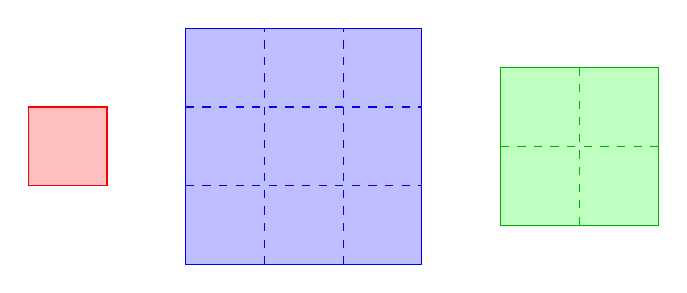
\begin{tikzpicture}
            \draw[red,fill=red!25] (0,0) -- (1,0) -- (1,1) -- (0,1) -- cycle;
            \draw[blue,fill=blue!25] (2,-1) -- (2,2) -- (5,2) -- (5,-1) -- cycle;
            \draw[green!70!black,fill=green!25] (6,-0.5) -- (8,-0.5) -- (8,1.5) -- (6,1.5) -- cycle;
            \draw[dashed,blue] (3,-1) -- (3,2);
            \draw[dashed,blue] (4,-1) -- (4,2);
            \draw[dashed,blue] (2,0) -- (5,0);
            \draw[dashed,blue] (2,1) -- (5,1);
            \draw[dashed,green!70!black] (7,-0.5) -- (7,1.5);
            \draw[dashed,green!70!black] (6,0.5) -- (8,0.5);
        \end{tikzpicture}
    \end{center}
    \begin{enumerate}
        \item Ordne den obigen drei Quadraten durch eine Abbildung $f$ mit expliziter Abbildungsvorschrift ihren Flächeninhalt zu (das rote Quadrat hat Seitenlänge $1$, das blaue Seitenlänge $3$ und das grüne Seitenlänge $2$).
        \item Eine Abbildung $g$ soll die Seitenlänge eines Quadrats auf den Flächeninhalt des Quadrats abbilden. Berechne $g(0), g(7)$ und $g(11)$.
        \item Gib für die Abbildung $g\colon\Natural\rightarrow\Natural$ eine Berechnungsvorschrift an.
        \item Kann die Abbildungsvorschrift von $g$ auch durch die explizite Schreibweise notiert werden?
    \end{enumerate}
\end{exercise}
\begin{exercise}{easy}
    \begin{wrapfigure}{r}{.4\textwidth}
        \centering
        \begin{tabular}{cc}\toprule
            Torschütze & Tore\\\midrule
            Anton &  3\\
            Max & 1\\
            Peter & 2\\
            Kai & 1\\\bottomrule
        \end{tabular}
    \end{wrapfigure}
    Die Fußballmannschaft, in der Peter spielt, hat ihr letztes Spiel haushoch mit 7:0 gewonnen. Der Verein hat anschließend die Tabelle mit den Torschützen veröffentlicht, die rechts zu sehen ist.
    \begin{enumerate}
        \item Welche Abbildung ist in der Tabelle dargestellt? Definiere die Abbildung formal mithilfe der expliziten Schreibweise für die Abbildungsvorschrift.
    \end{enumerate}
    Die Damen-Hockeymannschaft des Vereins hat im letzten Spiel ebenfalls sehr viele Tore erzielt und 5:1 gewonnen. Linda hat ein Tor erzielt, Nora und Anja haben jeweils zweimal getroffen.
    \begin{enumerate}[resume]
        \item Notiere auch für das Hockeyspiel formal eine Abbildung mit expliziter Abbildungsvorschrift.
        \item Erstelle eine Wertetabelle für die Tore der Hockeymannschaft, die die Abbildung aus b) darstellt.
    \end{enumerate}
\end{exercise}
\begin{exercise}{easy}
    In einer Bäckerei kosten Brötchen 30 Cent, Brezeln 80 Cent und Muffins 95 Cent.
    \begin{enumerate}
        \item Erstelle eine entsprechende Wertetabelle.
        \item Lies aus der Wertetabelle die Abbildungsregeln ab, um sie mit der expliziten Schreibweise zu notieren. Gib die Abbildung vollständig mathematisch an.
    \end{enumerate}
\end{exercise}
\begin{exercise}{easy}
    Die Abbildung $f\colon\textsc{Wirbeltiere}\rightarrow\{\text{Fische},\text{Reptilien},\text{Säugetiere},\text{Vögel},\text{Amphibien}\}$ ordnet Tierarten ihrer Wirbeltierklasse gemäß der Berechnungsvorschrift
    \[f(x)=\text{Wirbeltierklasse, zu der $x$ gehören}\]
    zu (\textsc{Tierarten} ist die Menge, die alle Tierarten enthält, die zu den Wirbeltieren gehören, z.B. Katzen, Haie und Adler).
    \begin{enumerate}
        \item Berechne $f(\text{Hunde}), f(\text{Schildkröten})$ und $f(\text{Falken})$.
        \item Erstelle eine Wertetabelle, in der du die Abbildung $f$ eintragen kannst und stelle die Abbildung in dieser Tabelle für die Argumente \emph{Igel, Goldfische, Antilopen, Laubfrösche} und \emph{Meisen} dar.
        \item Wie sieht die Abbildungsvorschrift für diese fünf Tiere in expliziter Schreibweise aus?
    \end{enumerate}
\end{exercise}
\begin{exercise}{easy}
    Jede der folgenden Wertetabellen stellt eine Abbildung von den ganzen Zahlen in die ganzen Zahlen dar, also eine Abbildung $f\colon\Integer\rightarrow\Integer$.
    
    \begin{multicols}{5}
    \begin{center}
        \begin{tabular}{cc}\toprule
            $x$ & $f(x)$ \\\midrule
            1 & 2\\
            2 & 4\\
            3 & 6\\
            4 & 8\\
            5 & 10\\
            \vdots & \vdots\\\bottomrule
        \end{tabular}
        \begin{tabular}{cc}\toprule
            $x$ & $f(x)$\\\midrule
            1 & 2\\
            2 & 3\\
            3 & 4\\
            4 & 5\\
            5 & 6\\
            \vdots & \vdots\\\bottomrule
        \end{tabular}
        \begin{tabular}{cc}\toprule
            $x$ & $f(x)$ \\\midrule
            1 & 0\\
            2 & 0\\
            3 & 0\\
            4 & 0\\
            5 & 0\\
            \vdots & \vdots\\\bottomrule
        \end{tabular}
        \begin{tabular}{cc}\toprule
            $x$ & $f(x)$ \\\midrule
            1 & 9\\
            2 & 8\\
            3 & 7\\
            4 & 6\\
            5 & 5\\
            \vdots & \vdots\\\bottomrule
        \end{tabular}
        \begin{tabular}{cc}\toprule
            $x$ & $f(x)$ \\\midrule
            1 & 10\\
            2 & 100\\
            3 & 1000\\
            4 & $10^4$\\
            5 & $10^5$\\
            \vdots & \vdots\\\bottomrule
        \end{tabular}
    \end{center}
\end{multicols}
    Gib für jede Wertetabelle die darin dargestellte Abbildung an. Schreibe die Abbildungsvorschrift dafür als Berechnungsvorschrift auf.
\end{exercise}
\begin{exercise}{easy}
    Ein Angler sitzt 5 Stunden lang an einem See und angelt Fische. Dabei fängt er durchschnittlich zwei Fische pro Stunde.
    \begin{enumerate}
        \item Definiere eine Abbildung, die der Anzahl der Stunden, die der Angler investiert, auf die Anzahl der Fische abbildet, die der Angler in dieser Zeit durchschnittlich angelt. Da der Angler nur 5 Stunden am See sitzt, genügt es, wenn du eine explizite Abbildungsvorschrift angibst, die nur die Argumente $0, 1, 2, 3, 4$ und $5$ Stunden abdeckt.
        \item Wir nehmen nun an, dass der Angler beliebig lang am See sitzt. Definiere durch eine Berechnungsvorschrift eine Abbildung, die die investierte Zeit des Anglers auf die Anzahl der Fische abbildet, die er angelt.
    \end{enumerate}
\end{exercise}
\begin{exercise}{easy}
    Das Wort \enquote{Fahrstuhl} hat zwei Vokale, das Wort \enquote{Ananas} drei. Die Abbildung \textsc{Vokale} soll beliebige Wörter auf die Anzahl der Vokale, die in ihnen vorkommen, abbilden.
    \begin{enumerate}
        \item Finde geeignete Definitions- und Bildmengen.
        \item Formuliere die Abbildungsvorschrift der Abbildung \textsc{Vokale} als Berechnungsvorschrift.
    \end{enumerate}
\end{exercise}
\begin{exercise}{easy}
    Die Abbildung $f\colon\Natural\rightarrow\Natural$ ist durch die Abbildungsvorschrift $f(x)=2^x$ definiert.
    \begin{enumerate}
        \item Gib $f(1), f(3)$ und $f(6)$ an.
        \item Erstelle eine Wertetabelle für $f$, in der du fünf beliebige Abbildungsregeln einträgst.
        \item Finde eine Zahl $x$, für die $f(x)=32$ gilt.
    \end{enumerate}
\end{exercise}
\begin{exercise}{easy}
    Notiere jeweils die Berechnungsvorschrift für eine Abbildung $f\colon\Real\rightarrow\Real$ mit der gewünschten Eigenschaft.
    \begin{enumerate}
        \item $f$ verdreifacht jede Zahl.
        \item $f$ bildet jede Zahl auf ihren Betrag ab.
        \item $f$ bildet alle Zahlen auf die Zahl $1$ ab.
        \item $f$ lässt jede Zahl so, wie sie ist (d.h. $f$ bildet alle Zahlen auf sich selbst ab).
    \end{enumerate}
\end{exercise}
\begin{exercise}{difficult}
    Finde eine Berechnungsvorschrift für eine Abbilding $f\colon\Natural\rightarrow\Natural$, die\dots
    \begin{enumerate}
        \item zu jedem Argument $x$ die größte gerade Zahl, die kleiner als $x$ ist, addiert.
        \item jede Zahl $x$ auf die Summe aller ungeraden Zahlen $n$ mit $1\leq n\leq x$ abbildet.
    \end{enumerate}
\end{exercise}
\begin{exercise}{difficult}
    Zwei natürliche Zahlen $n$ und $m$ heißen \textbf{teilerfremd}, falls es außer der $1$ keine Zahl gibt, die sowohl $n$ also auch $m$ teilt. Beispielsweise sind die Zahlen $4$ und $5$ teilerfremd, die Zahlen $4$ und $6$ hingegen nicht, weil man beide Zahlen ohne Rest durch $2$ teilen kann.
    
    Die \textbf{Eulersche Funktion} ist eine Abbildung $\varphi\colon\Natural\rightarrow\Natural$, die jeder natürlichen Zahl $n$ die Anzahl der Zahlen zuweist, die kleiner als $n$ und teilerfremd zu $n$ sind. $\varphi$ ist also durch die Berechnungsvorschrift \[\varphi(x)=\abs{\{n\in\Natural\:|\:n\leq x\text{~und~}n\text{~ist teilerfremd zu~}x\}}\] definiert.
    \begin{enumerate}
        \item Berechne $\varphi(6)$ und $\varphi(7)$.
        \item Finde eine einfache Berechnungsvorschrift, um $\varphi(p)$ für eine beliebige Primzahl $p$ auszurechnen.
        \item Es seien $p$ und $q$ Primzahlen. Berechne $\varphi(p\cdot q)$.
    \end{enumerate}
\end{exercise}
\begin{exercise}{difficult}
    Im Folgenden untersuchen wir eine Abbildung $f\colon\Integer\rightarrow\Rational$ mit der Eigenschaft, dass für alle $a,b\in\Integer$ die folgende Bedingung erfüllt ist:\[f(a)+f(b)=f(a+b).\]
    \begin{enumerate}
        \item Zeige, dass $f(0)=0$ sein muss.
            \hint{Es gilt $0=0+0$. Diese Eigenschaft kannst du in deinem Beweis verwenden.}
        \item Wir wählen ein beliebiges $n\in\Integer$. Wir bezeichnen $f(n)$ mit $m$, d.h. $m$ ist das Bild, auf das $n$ von $f$ abgebildet wird. Zeige, dass dann $f(-n)=-m$ gelten muss.
            \hint{Das Bild von der Summe $n+(-n)$ muss nach Aufgabenteil a) den Wert $0$ haben, weil $n+(-n)=0$ gilt.}
        \item Gib eine solche Abbildung an, für die nicht $f(1)=1$ oder $f(1)=0$ gilt.
        
        %\offerHint{7}{a}
        %\offerHint{4}{b}
    \end{enumerate}
\end{exercise}

\begin{exercise}{advanced}
    Im Folgenden untersuchen wir eine Abbildung $f\colon\Integer\rightarrow\Rational^*$ mit der Eigenschaft, dass für alle $a,b\in\Integer$ die folgende Bedingung erfüllt ist:\[f(a)\cdot f(b)=f(a+b).\]
    \textbf{Erinnerung:} $\Rational^*$ ist die Menge der rationalen Zahlen ohne $0$.
    \begin{enumerate}
        \item Zeige, dass $f(0)=1$ sein muss.
            \hint{Es gilt $0=0+0$. Diese Eigenschaft kannst du in deinem Beweis verwenden.}
        \item Gib eine solche Abbildung $f$ an, für die nicht $f(1)=1$ gilt.
        
        %\offerHint{7}{a}
    \end{enumerate}
\end{exercise}
\end{document}